\section{Soft Grasping Manipulator}
\label{sec:soft_grasping_manipulator}
\rkk{The robotic manipulator is composed of multiple bidirectional planar arm segments and combined with a unidirectional soft gripper.}
%We first introduce the previously developed uniform channel design, which is used for the soft body arm segments.
%Following this, 
We briefly describe the design, fabrication and functionality of this soft grasping manipulator in this paper. Further details on the design and fabrication can be found in \cite{marchese2015recipe}.

%\subsection{Uniform Channel Design of the Soft Arm}
%Several existing body segment morphologies are serpentine channels \cite{correll2010soft, marchese2014design}, uniform lateral channels \cite{marchese2014whole}, and pleated channels \cite{polygerinos2013towards, mosadegh2014pneumatic}.
%The serpentine channel design with its multiple vertical channels was first characterized by Correll et al.\cite{correll2010soft} and Onal et al.\cite{onal2011soft} and called a fluidic elastomer actuator.
%Several existing body segment morphologies are serpentine channels \cite{correll2010soft, marchese2014design}, uniform lateral channels \cite{marchese2014whole}, and pleated channels \cite{polygerinos2013towards, mosadegh2014pneumatic}.
%The serpentine channel design with its multiple vertical channels was first characterized by Correll et al.\cite{correll2010soft} and Onal et al.\cite{onal2011soft} and called a fluidic elastomer actuator.
%A cross sectional view of this design is shown in Figure~\ref{fig:design}-1.
%The design is described in \cite{marchese2014design} and paraphrased here.
%Bidirectional bending of this segment type is achieved by the pressurization of paired agonistic fluidic channel groups shown in \emph{yellow} that are separated by an inextensible but flexible constraint layer shown in \emph{black}. 
%These fluid channels are embedded within elastomer layers shown in \emph{cyan}.
%When a channel's internal fluid is pressurized, the elastomer deforms and the inextensible constraint transforms this channel deformation into segment curvature.
%The inextensible layer is typically made of a thin plastic film or fabric.
%A uniform channel design for soft segments is shown in Figure~\ref{fig:design}-1.
%It is an extension of the serpentine channel design by Correll et al. \cite{correll2010soft} and Onal et al. \cite{onal2011soft}. 
%The uniform channel design is achieved through changing both its kinematic constraints and fluidic channel geometry.
%This new design was first described in \cite{marchese2014whole} and is reused for our soft arm.
%The outer concentric layer remains composed of soft silicone rubber and is shown as \emph{transparent}.
%Bidirectional bending is achieved by pressurizing one of the two cylindrically-shaped and laterally embedded agonistic channels within this outer layer. 
%These channels are shown in \emph{yellow}.
%Also, a stiffer inner silicone layer shown in \emph{cyan} replaces an inextensible constraint layer found in the serpentine channel design.
%The stiffer inner layer introduces a partial constraint, so that an expansion of the lateral fluidic channels causes bending.
%This entirely soft design is simpler to fabricate because it does not require lamination.
%The design though is limited in defining the geometry of the fluidic channels, only cylindrical or cone shaped fluidic channels are possible. 
%This design is modular, because tubes can be passed through a hollow center, which allows the combination of many segments to an arm.
%Also, this design does not delaminate under high pressure as opposed to the serpentine design.
%This design was therefore chosen for making the arm to which the gripper is attached.

\begin{figure}[thpb]
\centering
   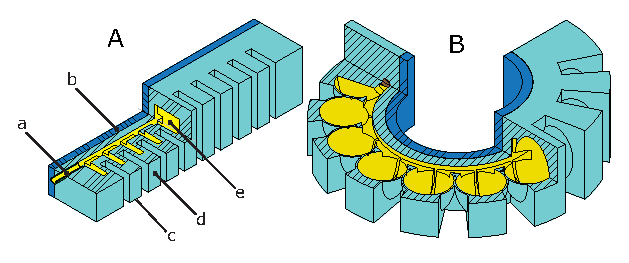
\includegraphics[width=0.99\columnwidth]{figures/robotic_gripper/design_gripper_detailed.eps}
   \caption{The pleated channel designs. The design consists of a channel inlet (a), an almost inextensible constraint layer (b), uniform pleats (d) separated by even gaps (c), and internal channels within each pleat (e). (\textbf{A}) depicts the segment in an unactuated state and (\textbf{B}) shows the segment in an actuated and therefore bent state. The expansion of the pressurized channels are schematically represented. \rkk{Reproduced from \cite{marchese2015recipe}.}}
   \label{fig:design}
\end{figure}


%\begin{figure}[!ht]
%\centering
%   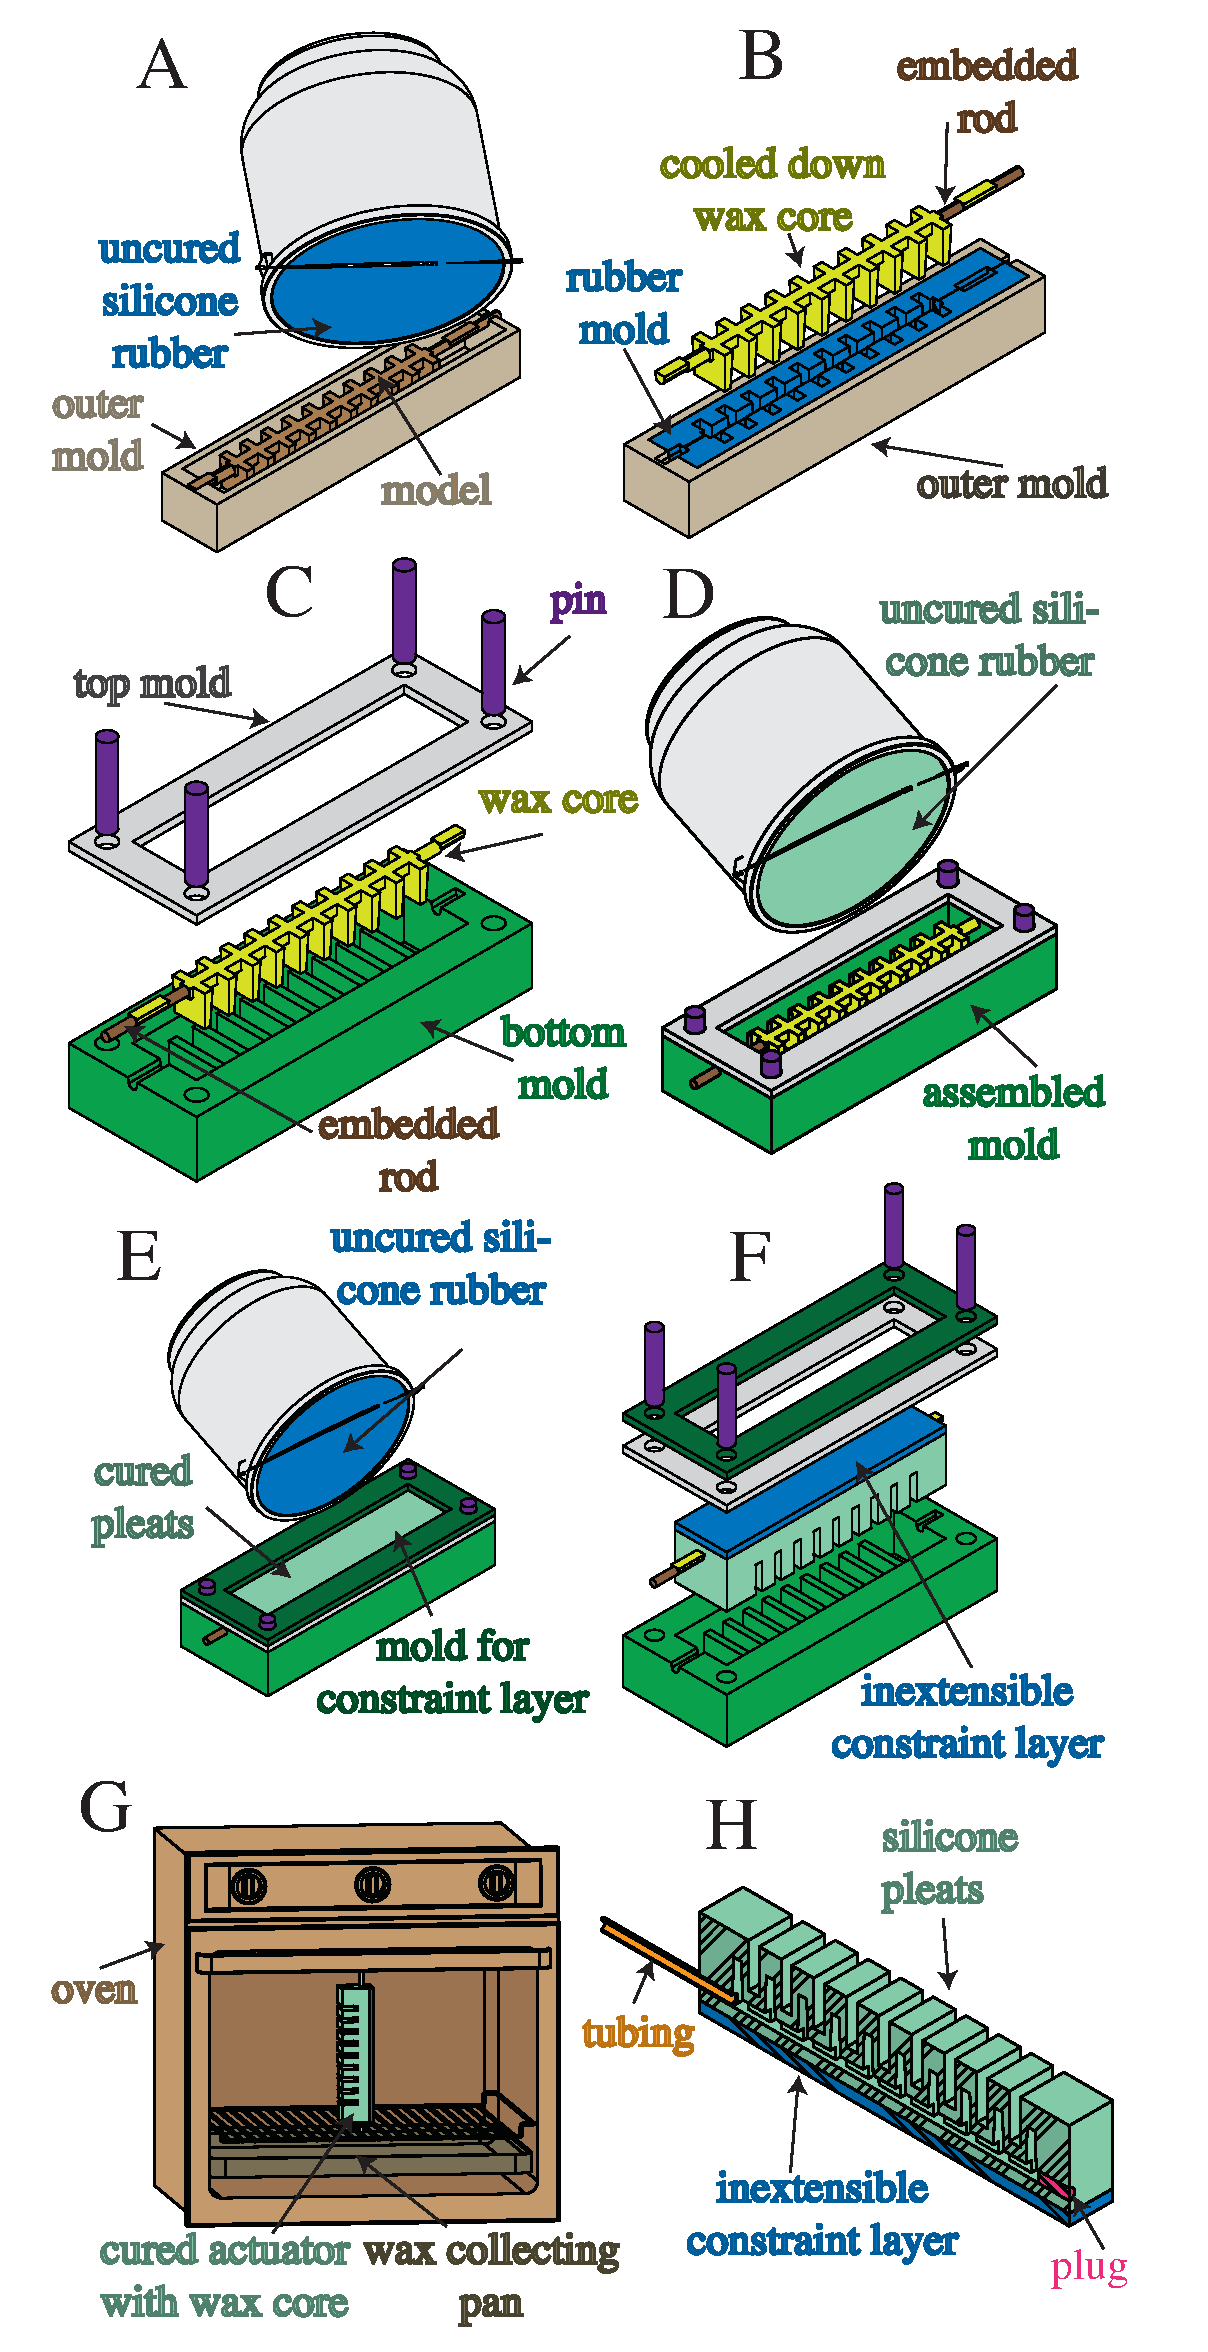
\includegraphics[width=0.85\columnwidth]{figures/robotic_gripper/fabrication_upright.eps} %fab_pleated_process_horizontal_no_labels.eps
%      \caption{Gripper fabrication process. (\textbf{A}) Pour and cure a rubber mold \rkk{(blue)}, (\textbf{B}) pour wax core \rkk{(yellow)} with embedded supportive rod \rkk{(brown)}, (\textbf{C}) combine bottom mold \rkk{(green)}, top mold \rkk{(grey)} and wax core using pins, (\textbf{D}) pour \rkk{softer} rubber \rkk{(light green)} into assembled mold, (\textbf{E}) pour stiffer rubber \rkk{(blue)} on top of the cured gripper \rkk{(light green)} to form a constraint layer, (\textbf{F}) remove cured gripper from mold, (\textbf{G}) using an oven melt out wax core from the gripper, and (\textbf{H}) add silicone tubing and plug using silicone sealant. \rkk{Reproduced from \cite{marchese2015recipe}.}}
%      \label{fig:fabrication}
%\end{figure}

\subsection{Pleated Channel Design for the Gripper}
The pleated channel design consists of evenly spaced ribs shown in \emph{cyan} with embedded hollow sections shown in \emph{yellow}.
Cut views of the un-actuated and actuated states are shown in Figure~\ref{fig:design}.
This design approach draws inspiration for its pleats from the soft pneumatic gloves developed by Polygerinos et al. \cite{polygerinos2013towards} and its homogeneous body design is inspired from the tail design of a soft robotic fish developed by Katzschmann et al. \cite{katzschmann2014hydraulic}.
This design is advantageous for grasping because it exhibits high curvature, minimal radial expansion, and remains compliant during actuation \cite{marchese2015recipe}. 
The hollow ribs within the segment's pleats are connected by a center channel and are accessible through a front inlet.
Under fluidic pressurization of the interior channel, an individual pleat allows for a ballon-like expansion of the thin exterior skin along the axial direction.
Similar to the uniform channel design, a stiffer silicone layer shown in \emph{blue} serves as an almost inextensible constraint layer.
The sum of the ballon-like expanding motions leads to bending of the less extensible center constraint layer to form a grasp.
The pleated design is capable of unidirectional bending up to extreme curvatures.
Using a lost-wax casting approach, we are not limited in defining the geometry of the segment's fluidic channels.
Using this approach, the \emph{cyan} portion of the pleated gripper can be cured in a single step, avoiding any weakening seams due to lamination.
%\rkk{Fabrication techniques based on the lamination of several cast rubber pieces lead to more manufacturing inconsistencies due to slight misalignments of layers. 
%We observed that soft actuators built this way tend to rupture more easily at their weakening seams.}

\subsection{Lost Wax Fabrication for Fluidic Elastomer Actuators}
Existing soft fluidic manipulators are mostly produced through a multi-step lamination process called \emph{soft lithography}, which results in weakening seams that can easily delaminate. 
This limits their range of applications and lifetime.
\rkk{The retractable pin fabrication for uniform lateral channels, first introduced in \cite{marchese2014whole},
limits the complexity of the cavities to cylindrical shapes but does not cause weakening seams to the actuator.}
%does not cause weakening seams to the actuator, but it also does not allow for cavities more complicated than cylindrical shapes.}
This is why the application of lost-wax casting to the fabrication of soft fluidic actuators like a gripper is advantageous.
The actuated cavities of the soft gripper are achieved using a wax core, pourable silicone rubber and 3D printed molds.
The gripper fabrication process and the tools needed are fully described and depicted in Section~4.3. and Figure~14 in \cite{marchese2015recipe}. %Figure~\ref{fig:fabrication}.
%The tools and equipment used are also listed in Table~\ref{tab:MachineTools} and are referred to by superscripts.
%
%In step (A), harder silicone rubber$^6$ is poured into a mold, which contains a 3D-printed model of the wax core.
%In preparation for step (B), the model is removed and the rubber mold is left inside the outer mold.
%A rigid rod is \rkk{embedded} as a supportive inlay inside the wax core.
%The rod is laid into the cavity of the rubber mold, supported on both ends by the outer mold.
%This ensures that the wax core does not break when removed from the rubber mold.
%\rkk{Mold release spray is applied to the silicone rubber mold to ease the wax core removal process.}
%The bees-wax$^{7}$ is heated up until it becomes fully liquefied.
%The assembly of rubber mold and outer mold is then heated up for a few minutes to the same temperature as the wax.
%Using a syringe, the liquid wax is injected into the assembly.
%Within a few minutes, the injected wax will start to solidify and significantly shrink in volume; this is counteracted by injecting more hot wax into the solidifying wax core during cool down.
%In step (B), the wax core is first allowed to completely cool down, then it is released from the mold.
%In step (C), the cooled down wax core is assembled together with the bottom mold, which defines the pleated structure of the gripper.
%The mold assembly is aligned with a top mold using pins. This top mold provides for additional volume to cover the wax core.
%In step (D), low elastic modulus rubber$^1$ is mixed, degassed in a vacuum$^2$, and poured to form the gripper and allowed to cure.
%In step (E), stiffer rubber$^3$ is poured on top of the cured gripper to form a constraint layer.
%In step (F), the cured gripper is removed from the mold.
%In step (G), most of the wax core is melted out by placing the gripper into an oven in an upright position.
%After this, remaining wax residues are cooked out in a boiling water bath.
%Finally, in step (H) a silicone tube$^5$ and a piece of silicone cord$^{8}$ get covered with silicone sealant$^4$ and are inserted into the front and back holes respectively.
%
%\begin{table}[h]
%\caption{Commercially Available Tools and Equipment}
%\centering
%\begin{tabular}{c l l}
%\hline
%\hline
%\# & Product Name & Company\\
%\hline
%1 & Ecoflex 0030&  Smooth-On\\
%2 & AL Cube & Abbess Instr. and Sys., Inc.\\
%3 & Mold Star 15 & Smooth-On\\
%4 & Silicone Sealant 732 & Dow Corning Corp\\
%5 & PN 51845K53 & McMaster\\
%6 & Mold Star 30 & Smooth-On\\
%7 & Beeswax & Jacquard\\
%8 & PN 9808K21& McMaster\\
%\hline
%\end{tabular}
%\label{tab:MachineTools}
%\end{table}

\subsection{Multi-segment Arm with Gripper}

The design for the arm consisting of soft cylindrical segments is described in \cite{marchese2014whole}.
\rkk{As is shown in \cite{marchese2015recipe} through the characterization of various actuator morphologies, the concatenation of soft cylindrical segments is most suitable to build up a robotic arm that can create high blocking forces per fluid energy inserted.}
 \rkk{The cylindrical segments of the arm are fabricated through a retractable pin fabrication technique \cite{marchese2014whole}, which does not require lost wax cores because of their simple cylindrical cavities.} 
Each cylindrical segment can be actuated up to a bend angle of about $60^\circ$, this requires several segments to be combined together to allow the arm to reach a large enough workspace to perform proper manipulation tasks on a plane. 
\rkk{Using six segments, the robot is able to touch its tip to its base without interference from the individual joint limits.}
%the joint limits do not prohibit the robot to reach with its tip its own root.} %Calculating the forward kinematics, see \texttt{forwKin()} in Algorithm~\ref{alg:planGrasp}, for the 6 DOF arm with a segment length of 6.27\unit{cm} and an extreme curvature of $\kappa = \frac{60/180 \pi}{0.0627\unit{m}} = 16.7\frac{1}{\unit{m}}$ shows that the tip of the robot can reach its root at a full curl.}
The cylindrical segment design with its hollow channel in the center has enough space to accommodate for pneumatic tubes to connect to all six cylindrical segments and additionally to the pleated gripper, which is attached to the tip. 
The pleated gripper has to be appropriately sized, just big enough to allow for proper manipulation without exceeding the payload capacity of the soft arm.

\rkk{The complete multi-segment arm is supported off the ground with two roller supports per segment. 
The rollers minimize frictional forces to the surface. 
If the arm would be moved over a non-slippery surface without rollers, the frictional effects would greatly reduce the agility of the arm and largely increase the stick-slip friction effects with the ground, rendering the arm less useful.}
